\chapter{研究概要}
\label{introduction}

\section{序論}

産業革命、そしてコンピュータによる情報革命と、人々が道具や機械を発展させる中、ヒューマンインターフェースを設計する必要が生じた。そこでの人と機械の最適な関係とは「より使いやすく有用に」\footnote{国際標準化機構(ISO)による「人間中心設計」の導入部\cite{hcd}より}することとされ、エルゴノミクス、人間中心設計といった方法論がそれを具現化してきた。しかし、人と道具の関係とは果たして、私たちが「より使いやすく有用に」、一方的に使用するような関係だけだっただろうか?

ピアノを初めて弾くとき、奏者は手の大きさによる制約を受け、最初のうちは左右別々に指を動かすだけでも困難さを経験する。しかし、試行錯誤を経て、ピアノの制約と自身の身体能力との間で折り合いをつけていくことで、ようやく楽器を通して表現ができるようになる。ミュージシャンのスキャットマン・ジョン(ジョン・ポール・ラーキン)は、「吃音症」という発話障害を抱えながらも、「自身の身体」という切っても切り離せない存在をコントロールできない中、むしろその症状を逆手に取るように「テクノスキャット」という独自の歌唱法を開拓した。他者性と向き合う中で、自分なりの扱い方を見出していく過程とは、創造的で喜びのあるものであるはずだ。

Sydney Felsは、人とある対象との関係性について、「Embodiment:一体感」と「Intimacy:親密さ」の観点から幅広く説明する。その中には、「人が対象を自分の一部として取り込むことによる一体感」、今HCIや認知科学の領域で一般的に用いられる意味でのEmbodimentに重なるものがある一方で、興味深いことに「対象に人が取り込まれることによる一体感」にも言及している。こう聞くとなかなか想像しづらいが、これは例えばバイクに乗る人が、「バイクに合わせた走り方をする」ことや、楽器の演奏者がその楽器の特性にあわせて、いわば楽器に翻弄されるように演奏する中で得られる一体感を指している。そして、こうした一体感を通して人とその対象とのあいだに「Intimacy:親密さ」が生まれるという。これこそが、ピアノなどに見られる、見落とされてきた関係性ではないだろうか?

しかし「より使いやすく有用に」作られたものに(少なくとも、作り手が意図した使い方の範疇では)、Felsのいう「対象に人が取り込まれることによる一体感」が生じるとは考え難い。なぜならFelsが説明するように、この一体感は「人が自身の統制力を手放す」ことで生じるからだ。\footnote{"In this situation, the person derives an aesthetic feeling through relinquishing control of themselves so that the object can manipulate them.(このような状況下では、人は対象が自分を操作できるように、自身の統制力を手放すことで美的感覚を得る。)\cite{Fels}"}「より使いやすく有用に」作られた道具に向き合う状況とはむしろ、対象に「統制力」を不自由なく行使できる状況である。対象はたちまち身体と一体化し、「透明」になる。「透明」になった対象に影響を受けながら、折り合いをつけていくことは起きづらい。

では、楽器やバイクに見られる、いわば「人馬一体」と言われるような、相互の折り合いをつけながら生まれる親密さはどのように生まれ、そうした関係性が芽生える状況とはいかに設計できるのか。Felsはこうした関係性を捉える重要な枠組みを提示したが、具体的にどのようにしてそれが達成されるのかについては説明していない。

ここでは、それを捉えるための枠組みとして\textit{grasp}という概念、噛み砕いて言えば人があるものに対して「手探りでなにかを掴もうとする態度」を定義し、それがどのように具現化するのかを探求するプロジェクトとして、修士作品《Grasp(er)》を制作した。本研究では、この作品の制作プロセスと、体験について詳細に分析することを通して、\textit{grasp}をどのように適用していけば、この親密さが起こるのかについて考察する。

\section{問題提起}
\label{subject}
人間が使用する道具に機械や情報処理が介在し、高度で複雑なシステムになった現在、人間と道具との関係をいかに設計するか、すなわちヒューマンインターフェースデザインが重要視となった。その理想とは、原始的な道具の使用感と同じように、原因と結果の対応が直接的であり、その道具を使っているという意識がなくなる「道具の透明化」であるとされてきた\cite{Watanabe2017}。インターフェース研究者の渡邊は、その理想を実現する指針として「自己帰属感」
\footnote{「自己帰属感」は、Gallagherの「ミニマルセルフ」における「Sense of Ownership」に対して渡邊が用いた訳語である\cite{Watanabe2017}。認知科学者・哲学者のGallagherは、自己を構成する2つの要素として、ミニマルセルフ(最小限の自己)とナラティヴ・セルフ(物語的自己)があると説明した\cite{Gallagher2000}。中でも「ミニマルセルフ」とは、一切の自己知識を失ったとしても残る最小限の自己であり、身体所有感(sense of ownership, body ownership)、行為主体感(sense of agency)の二つによって支えられていると説明する。こうしたGallagherの分類に基づき、それらを評価する方法が考案され、ラバーハンド錯覚実験などにみられるように、生来の肉体ではないものを自分の身体と錯覚してしまうような、人間の身体像の曖昧さに注目した研究が認知科学や心理学の領域で取り組まれてきた。}
という概念を導入し、例えばマウスカーソルやスマートフォンのような「操作時の指とグラフィックの追従性が高い」インターフェースは自身の一部や延長として感じられる、「透明」なインターフェースであると説明する。

確かにこうしたインターフェースを設計していくことは、複雑で高度な道具の力を借りて人間の活動の可能性を拡げることに貢献してきた。しかし人間と道具の関係とは果たして、人間が一方的に使用するような関係だけだっただろうか?渡邊の「自己帰属感」とは、使い手である「自己」がいて、その自己が思い通りに対象を使用できるよう、対象が自己に「帰属」する感覚についての説明である。その逆に、対象に自己が歩み寄っていくような関係について、少なくともインターフェースの設計において議論されることは少ない。しかしそうした関係は、身近に存在している。

ピアノを初めて弾くとき、奏者は手の大きさによる制約を受け、最初のうちは左右別々に指を動かすだけでも困難さを経験する。しかし、試行錯誤を経て、ピアノの制約と自身の身体能力との間で折り合いをつけていくことで、ようやく楽器を通して表現ができるようになる。ミュージシャンのスキャットマン・ジョン(ジョン・ポール・ラーキン)は、「吃音症」という発話障害を抱えながらも、「自身の身体」という切っても切り離せない存在をコントロールできない中、むしろその症状を逆手に取るように「テクノスキャット」という独自の歌唱法を開拓した。他者性と向き合う中で、自分なりの扱い方を見出していく過程とは、創造的で喜びのあるものであるはずだ。

コンピュータ工学研究者のSydney Felsは、対象と人との関係性を、「Embodiment」の観点から4つに分類した\cite{Fels}。Embodimentとは日本語で「身体化、一体化、身体性」などと訳されるが、動詞の「embody」についてCambridge Dictionaryで引くと、"\textit{to include as part of something} ((何かを)何かの一部として取り込むこと)"とある\cite{embody}。ここで指摘したいのは、Embodimentの原義は「何かを取り込んで、何かの一部とすること」であり、「人がオブジェクトを取り込んで、一体化すること」のみを指すわけではないということだ。

しかし、Embodimentという言葉はHCIの分野でも用いられ、その文脈でのEmbodimentとは「使い手である人に、対象が取り込まれる」という意味でのEmbodimentである\cite{veq}。

FelsのEmbodimentにおいて特徴的なのは、「人が対象を取り込む」一体化だけでなく、「対象が人を取り込む」という逆向きの一体化についても論じていることである。この「対象が人を取り込む」という逆向きの関係性について、これまで注目されることは少なかったのではないかと考える。

一方的に使用するだけでなく、対象からの影響について折り合いをつけながら一体化していくような、いわば「人馬一体」のような一体感とはどのように生まれ、そしてそうした関係性が芽生える状況とはいかに設計できるのか。本研究では、こうした問いにアプローチしていくことを目指した。

\section{研究概要}
本研究では、人間と道具や機械との関係において、人にとって道具や機械が「より使いやすく、有用に」あるという関係ではない、対象の他者性と向き合い、折り合いをつけていく経験を通して生まれる「一体感」を目指し、それがどのように生まれるのかについて探求する。この意味での「一体感」とは例えば、ピアノの演奏やバイクの運転など、人間が道具や機械の特性を理解し、使いこなすための能力を身につけることで生じる人間と対象との関係である。

この主題に、手指の変換を通して「身体の中の他者性」を経験させる表現を探索することから迫り、修士作品《Grasp(er)》を制作した。
また、人間と対象との関係について「Embodiment:一体化」の観点から分類したSydney Felsの4つのカテゴリやIntimacyの概念に基づき、本研究では\textit{grasp}という概念を提案した。この概念を用いて本作から「一体感」が生じるまでの過程についての仮説を立て、4名の作品体験を振り返ることから、それが実現しているかについて考察する。

\section{本研究の目的}
本研究の目的は、対象の他者性と向き合い、折り合いをつけていく経験を通して生まれる「一体感」について、それがどのように生じるのかについての詳細な説明と、そのために導入された概念である\textit{grasp}の妥当性を示し、そうした関係性が生じるものについての設計の指針を示すことである。

\section{リサーチクエスチョン}

これらの言葉を用いて本研究における問いを説明すると、次のようになる。

\begin{quote}
\textbf{対象からの影響も受けつつ(Belonging)、相互の折り合いをつけながら生まれる一体感(Intimacy)はどのように生まれ、そうした関係性が芽生える状況とはいかに設計できるのか。}
\end{quote}

本研究では、「手指の変換」を通して「身体の中の他者性」を経験させる表現を探索することからこの問いに迫った。

% この「手指の変換」という表現については、この問いの着想のきっかけでもある。こうした探索的なリサーチを通して、修士作品《Grasp(er)》と、それを説明するための\textit{grasp}という概念を示した。

\section{「手指の変換」に取り組む動機}
\label{prototyping_concept_making}
この問いは、もともと抱いていた\ref{subject}節のような問題意識に対して、当初はその問題意識とは無関係に進めていた「動きのスケッチツール」という目的の習作「Digitalize」を展示した際の体験者の様子が、その切り口になると捉えたことがきっかけとなって着想した。この節では、そうした着想に至るまでの経緯について説明することで、「手指の変換」からこの問いへアプローチすることの動機とする。

ここで制作した「Digitalize」とは、手指の動きを別の形へとマッピングさせた3つの変換表現から構成された作品である。

静止画について構想を膨らませる際、「紙とペン」を通して直接イメージをスケッチできるが、動きについてはそれに相当するほど、直感的かつ、高い表現力でスケッチができるツールが見当たらなかった。そこで、動きに関して高い表現力を有する手指の動きを使って、「動きをスケッチする」ツールを設計することを案じていた。

しかし手指は人間の身体の中でもとりわけ随意に、高い表現力で動かすことのできる器官である。もし「手ではない形」を通してでも、様々な形や動きを自由に作れるのなら、人間の身体構造による制約を超えた「動きのスケッチ」ができるのではないか。

そうして、手指の動きをトラッキングしつつ、画面上でその動きは別の形へマッピングされて動くインターフェースについて、プロトタイピングを行い、その過程をIAMAS Open House 2022にて展示した。この時点では、動きを記録する機能は存在しておらず、あくまで手と、それに伴って動く手指とは異なる形の動きが確認できるだけのものであった。

\begin{figure}[H]
  \centering
  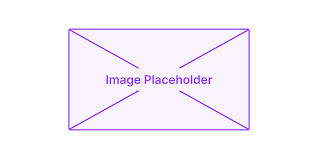
\includegraphics[width=15cm]{img/placeholder.png}
  \caption{IAMAS Open House 2022での展示の様子(2022年)}
  \label{fig:exhibit_2022}
\end{figure}

しかし展示を行うと、この試作には当初想定していなかった魅力があることに気づいた。それは、指の動きが単に、別の構造にマッピングされただけであるのに、別の構造の手を動かす体験はそれだけで興味を惹くものだということである。手指の変換が3パターン展示された状態のこの展示で、10分以上興味を持って体験する方が複数名いた。また、制作されたプロトタイプを展示した際、指先を動かすだけでなく、カメラに対して手を近づけたり遠ざけたり、手を裏返したりするなど、さまざまな体験の方法が現れた。

これは、「手指の動きに反応している」ということは分かっていても「どのように対応しているのか」がはっきりせず、それを確かめるように身体を動かしていると考えた。

仕組みを知っている制作者にとっては自明なことだが、自己の運動とどう対応するのかを知り得ない体験者は、自身の体を動かして観察されたことを通して推測することになる。それゆえに、この仕組みを通して思い描く身体像に、体験者ごとに違いがあるのではないか。

こうした体験者ごとの違いは、「わかりやすい」ものを対象としたときよりも、「わかりにくい」ものを対象としたときの方が顕著に現れると考えた。その上で、わかったようで分からない、行きつ戻りつな感覚に陥りながらも「わからなかった」と一蹴されず、それを分かろうとして向き合う様子が続いたことに、先の問題意識に応えるものがあるのではないかと考えた。

\section{本論文の構成}
本章では、研究の概要を示した。

第\ref{related_works}章では、研究背景について問題提起の形で示し、その上でリサーチクエスチョンを提示する。また、その問いを探索する切り口として本研究が着目した「手指の変換」について、その観点から取り組む動機、そして関連研究との相違点を説明することから研究の位置付けを明らかにする。

第\ref{about_grasper}章では、作品概要と、そこに至るまでのプロトタイピングの分析を通して、作品形態について説明する。

第\ref{graspについて}章では、本研究が提示するコンセプトである\textit{grasp}について詳細に説明する。その上で、Felsの分類との関係性と、この概念を用いることから修士作品の体験についてのねらいを説明する。

第\ref{validation}章では、そのようなねらいのもと制作された本作品が、実際どのように経験されるのかについての質的調査を行うため、Video Cued Recallという手法を用いて体験について振り返り、実際の体験がどのようなものであったのかを踏まえて、モデルとの関係性について考察する。

第\ref{考察}章では、行った調査の結果からどのような体験の作品であったかを振り返り、本作品が狙いとしていたこと、あるいはその範疇を超えて、作品として何が達成されたのかについて考察する。

第7章では、これまでの議論をまとめ、最後に今後の展望として、ここで制作を行ったモデルがそれ以外の議論とどのように関係し、今後どのような可能性を有するのかについて述べる。